\section{References}
\begin{frame}
\frametitle{References}
\begin{itemize}
  \item IEEE Computer Society. Software Engineering Technical Committee. (1993). \textit{IEEE Standard for a Software Quality Metrics Methodology}. Institute of Electrical and Electronics Engineering.
  \item Basili, V. R. and Weiss, D. M. (1984). A methodology for collecting valid software engineering data. \textit{Software Engineering, IEEE Transactions on}, (6):728–738.
  \item Parr, T. (2013). \textit{The Definitive ANTLR 4 Reference}. Oreilly and Associate Series. Pragmatic Bookshelf.
  \item Washizaki, H., Namiki, R., Fukuoka, T., Harada, Y., and Watanabe, H. (2007). A framework for measuring and evaluating program source code quality. In \textit{Product-Focused Software Process Improvement}, pages 284–299. Springer.
\end{itemize}
\end{frame}

\begin{frame}
\frametitle{References}
\begin{itemize}
  \item Fowler, M. (2014). Microservices. Retrieved March 20, 2016, from http://martinfowler.com/articles/microservices.html.
  \item Saff, D. and Ernst, M. D. (2005). Continuous testing in eclipse. In \textit{Proceedings of the 27th international conference on Software engineering}, pages 668–669. ACM.
\end{itemize}

\end{frame}

\begin{frame}
\label{appendix:software_quality_attributes}
\frametitle{Appendix: Software Quality Attributes}

A list of software quality attributes:
\begin{example}
\begin{multicols}{2}
\begin{itemize}
  \item Maintainability
  \item Efficiency
  \item Reliability
  \item Availability
  \item Correctness
  \item Fault-tolerance
  \item Interoperability
  \item Scalability
  \item Responsiveness
  \item Testability
  \item Usability
\end{itemize}
\end{multicols}
\end{example}

\hyperlink{subsection:software_quality}{\beamerreturnbutton{Back}}

\end{frame}

\begin{frame}
\label{appendix:software_quality_metrics}
\frametitle{Appendix: Software Quality Metrics}

A list of software quality metrics:
\begin{example}
\begin{multicols}{2}
\begin{itemize}
  \item Number of children
  \item Coupling between object classes
  \item Response for a class
  \item Lack of cohesion in methods
  \item Method hiding factor
  \item Attribute hiding factor
  \item Method inheritance factor
  \item Attribute inheritance factor
  \item Polymorphism factor
\end{itemize}
\end{multicols}
\end{example}

\hyperlink{subsection:software_quality_metric}{\beamerreturnbutton{Back}}

\end{frame}

\begin{frame}
\label{appendix:goal_question_metric}
\frametitle{Appendix: Goal Question Metric}

\begin{example}
\begin{tabular}{ l l }
Goal &: Testability \\
Question &: Is the size of the code reasonable? \\
Metrics &: Line of codes\\
\end{tabular}
\end{example}

\begin{example}
\begin{tabular}{ l l }
Goal &: Analysability \\
Question &: Are the naming of variables good? \\
Metrics &: Average length of identifier\\
\end{tabular}
\end{example}

\hyperlink{subsection:goal_question_metric}{\beamerreturnbutton{Back}}

\end{frame}

\begin{frame}[allowframebreaks]
\label{appendix:sonar_qube}
\frametitle{Appendix: SonarQube}

\begin{center}
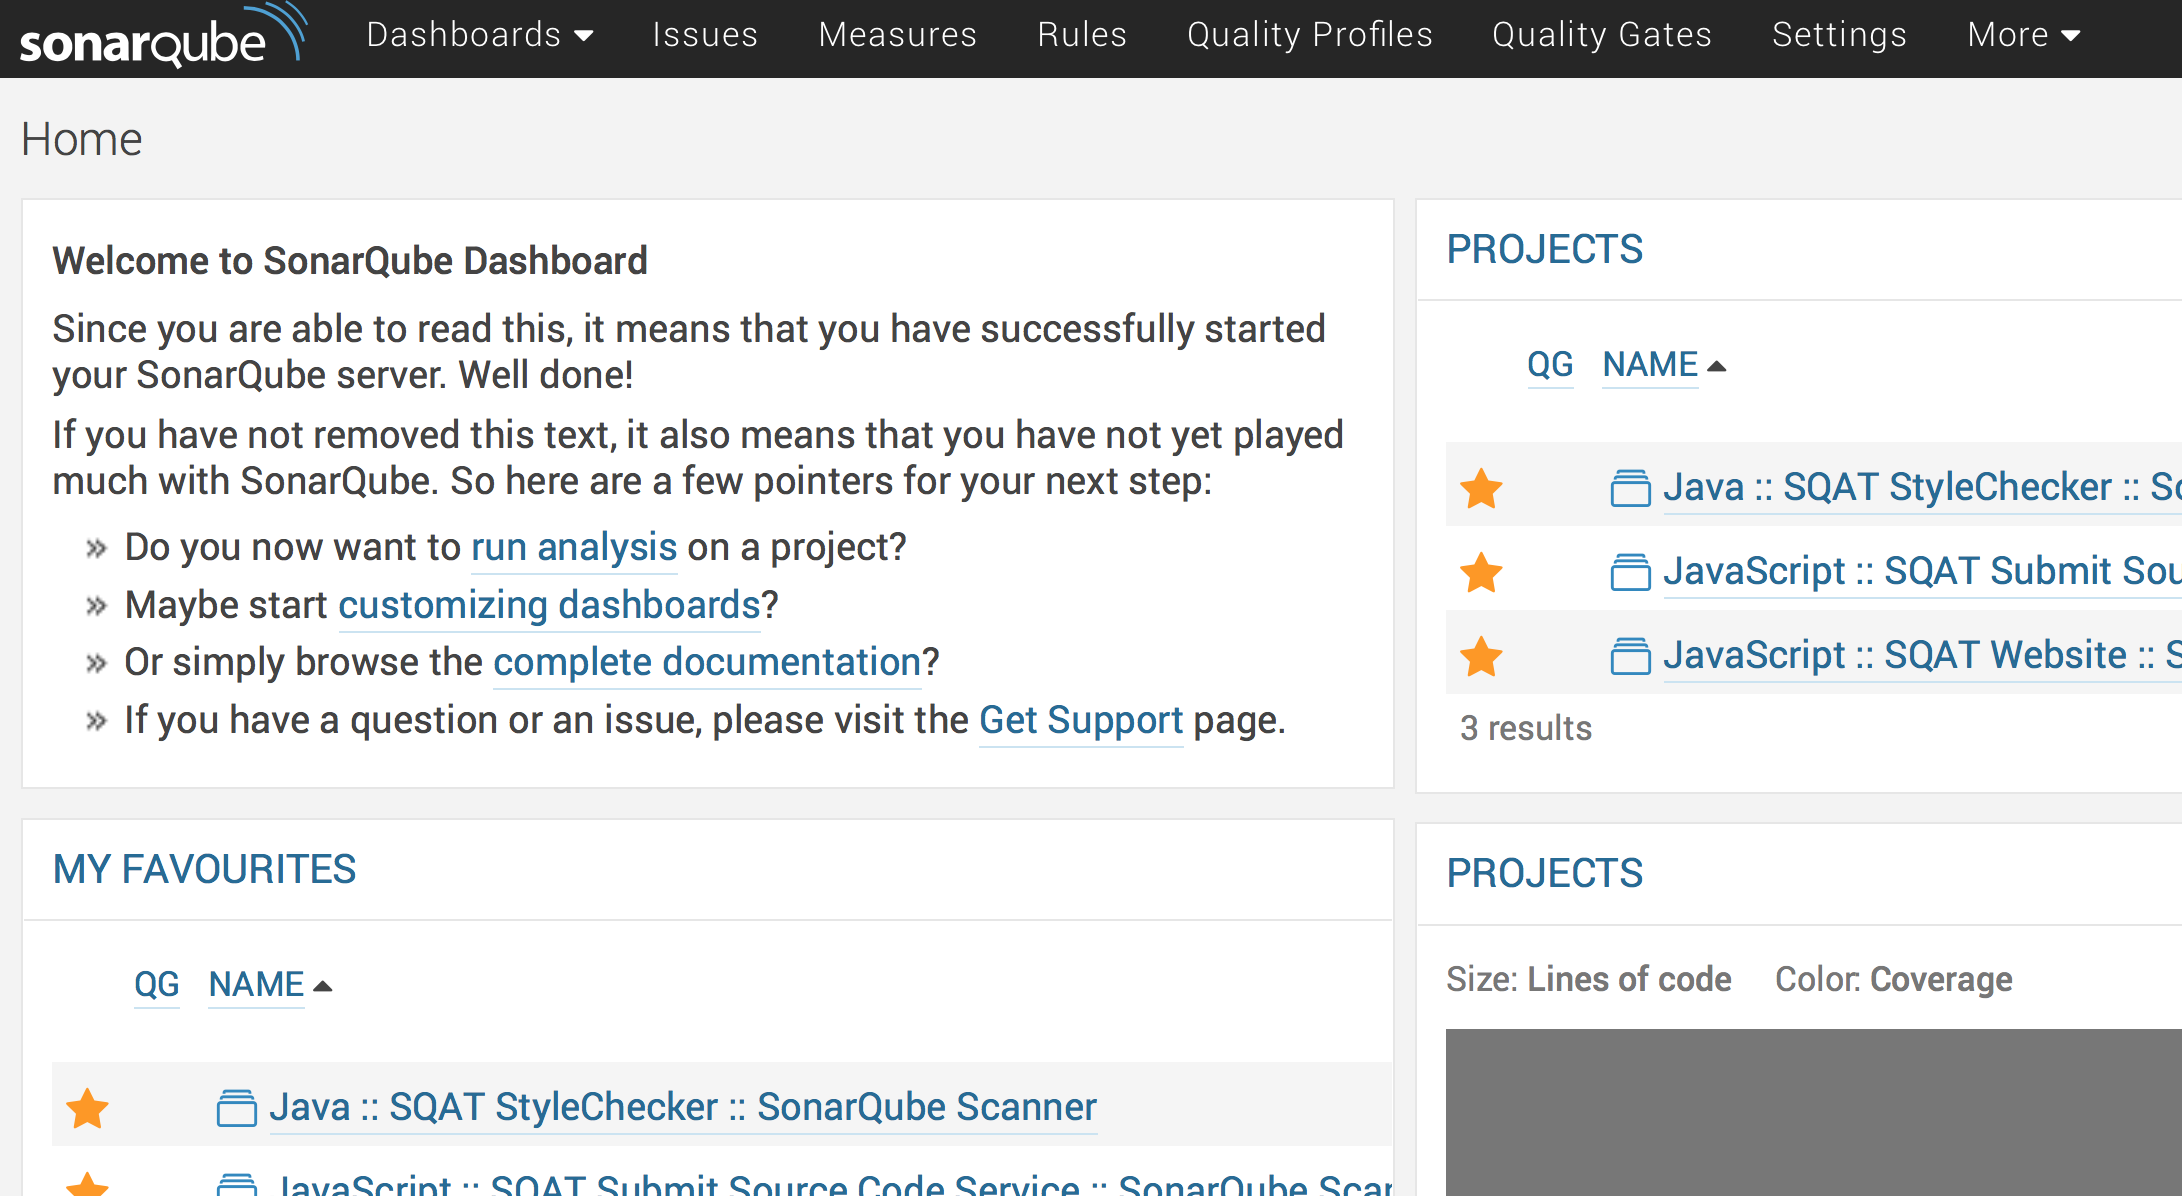
\includegraphics[width=\textwidth,height=0.7\textheight,keepaspectratio]{sonar_dashboard}
\end{center}
\hyperlink{subsection:sonar_qube}{\beamerreturnbutton{Back}}

\framebreak

\begin{center}
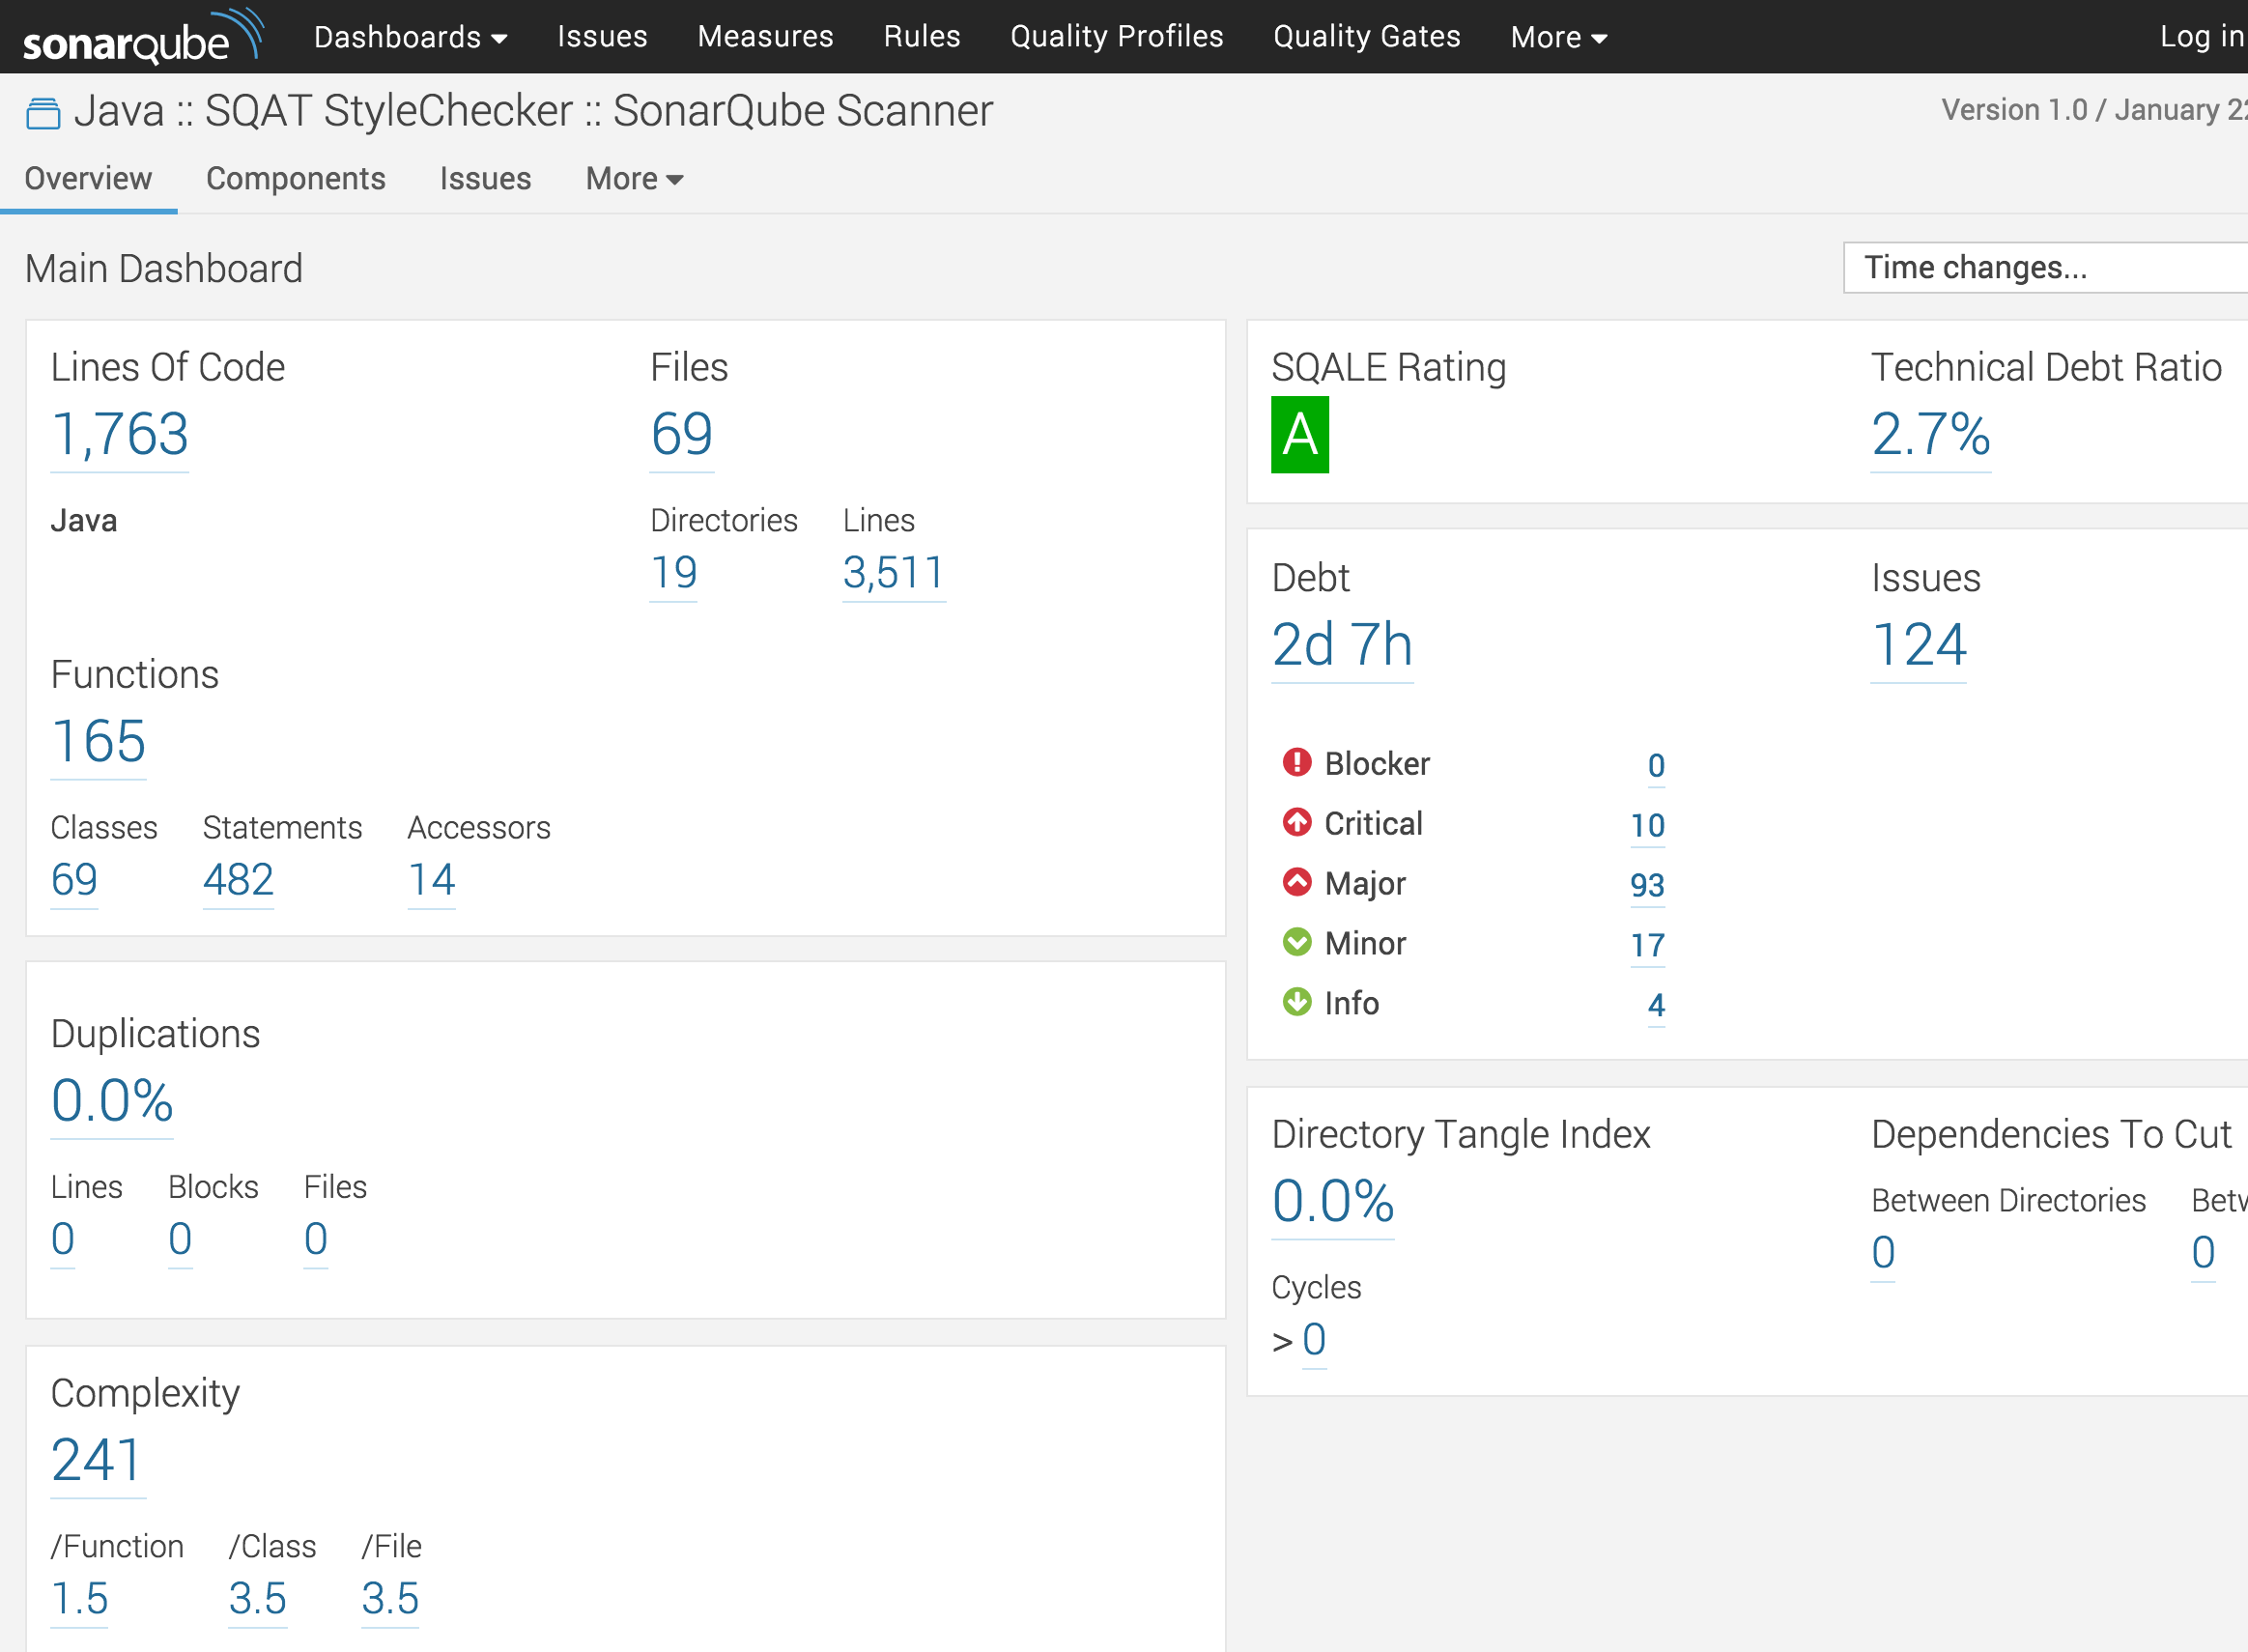
\includegraphics[width=\textwidth,height=0.7\textheight,keepaspectratio]{sonar_project_dashboard}
\end{center}

\hyperlink{subsection:sonar_qube}{\beamerreturnbutton{Back}}

\framebreak

\begin{center}
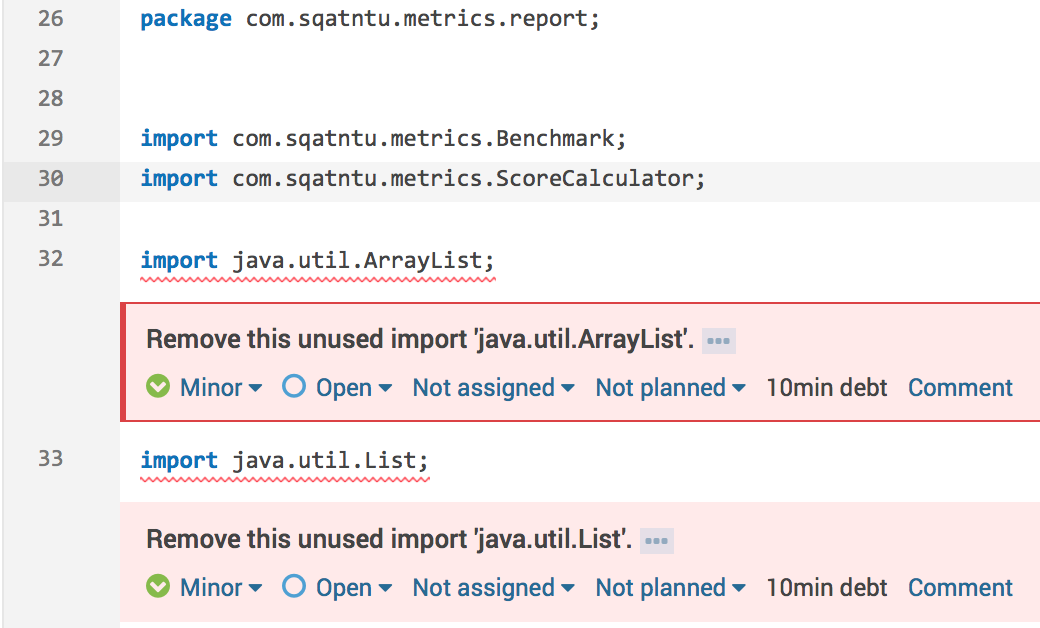
\includegraphics[width=\textwidth,height=0.7\textheight,keepaspectratio]{sonar_code_issue}
\end{center}

\hyperlink{subsection:sonar_qube}{\beamerreturnbutton{Back}}
\end{frame}

\begin{frame}[allowframebreaks]
\label{appendix:monolithic}
\frametitle{Appendix: Monolithic Architecture}

\begin{definition}
Monotolithic architecture is made up of multi-tier components, with components in upper tier use components in lower tier to perform some functions.
\end{definition}

The architecture has three major drawbacks:
\begin{itemize}
  \item Requires long-term commitment to a particular technology stack
  \item Difficult for developers to understand the whole application
  \item Difficult to scale an application horizontally
\end{itemize}

\hyperlink{subsection:overall_architecture}{\beamerreturnbutton{Back}}

\framebreak

\begin{center}
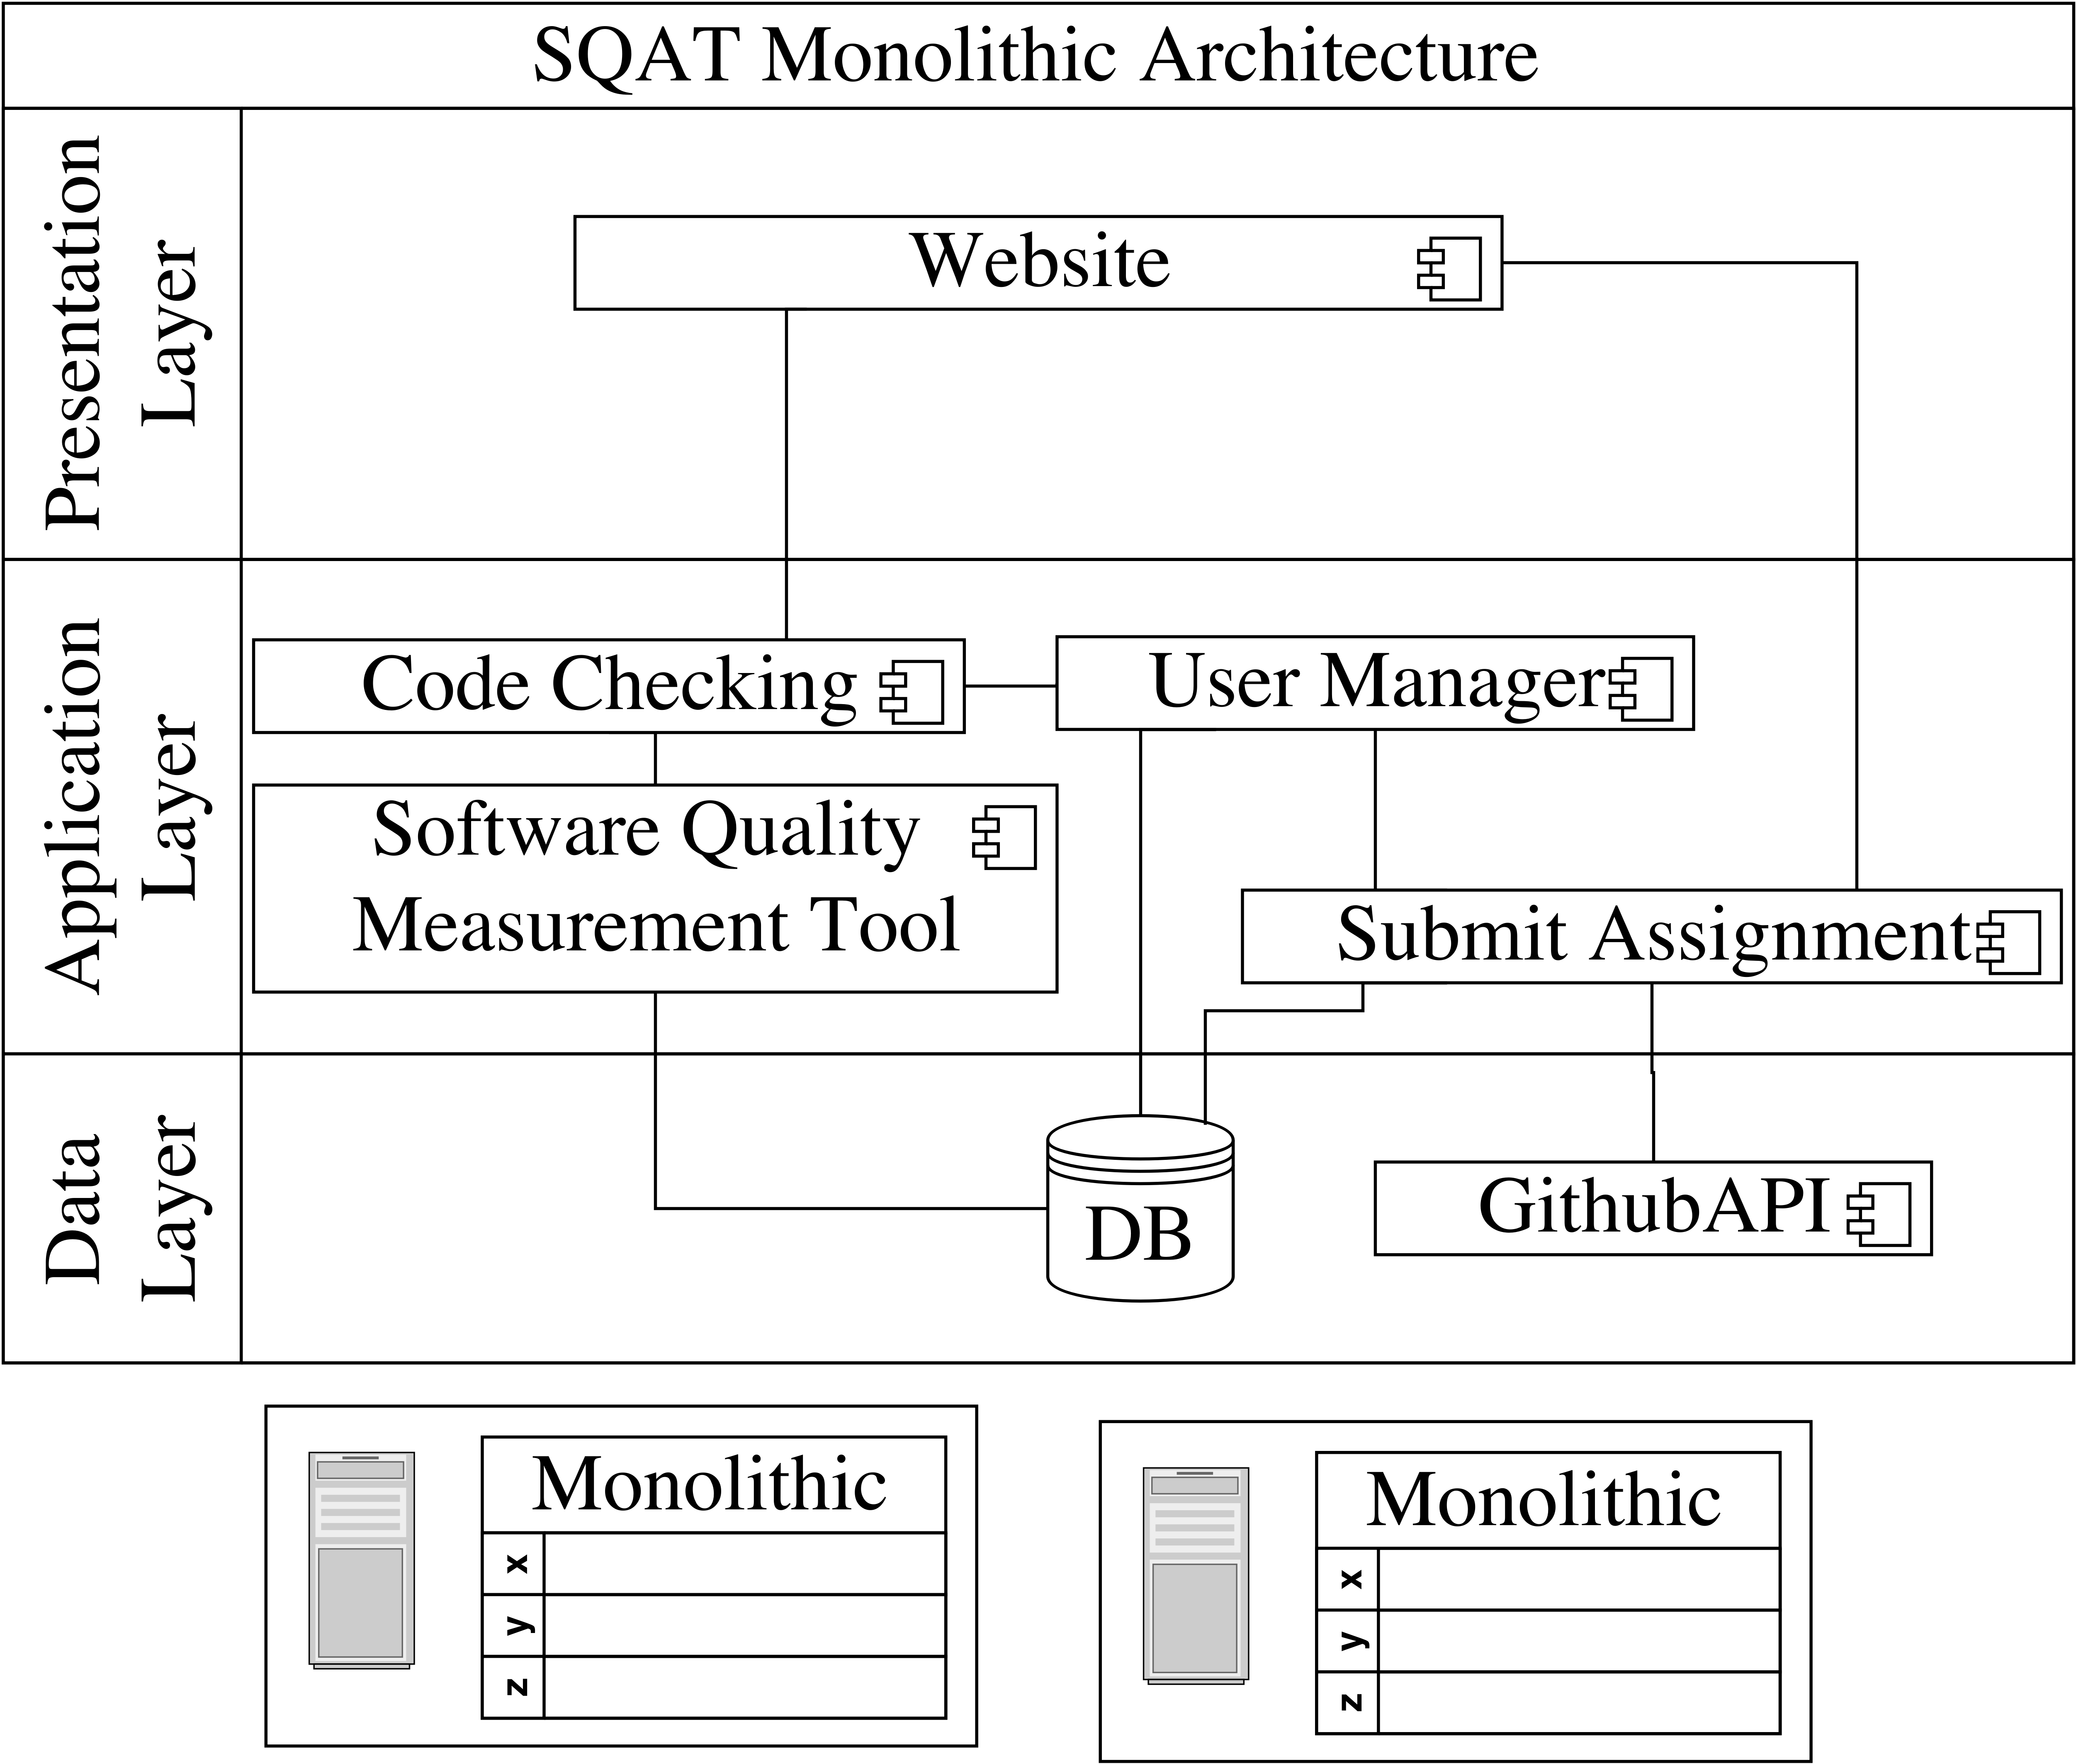
\includegraphics[scale=0.045]{SQAT_monolithic}
\end{center}

\end{frame}